\documentclass{beamer}
\usepackage[utf8]{inputenc}

\usepackage{tikz}

\title{gPTP (IEEE802.1AS) - Standard for Local and Metropolitan Area Networks - Timing and Synchronization for Time-Sensitive Applications in Bridged Local Area Networks}
\author{Marvin Gnad}

\begin{document}
\frame{\titlepage}

\begin{frame}
\frametitle{Why? How? What?}
\begin{itemize}
    \item NTP is not accurate enough for real time applications
    \item Establishing a clock where several participants in a local network can refer to
    \item PTP is used for local domains e.g. festivals, concert, car infotainment
    \item Ethernet hardware needs to support this feature
\end{itemize}
\end{frame}

\begin{frame}
\frametitle{Clock synchronisation}
\begin{center}
    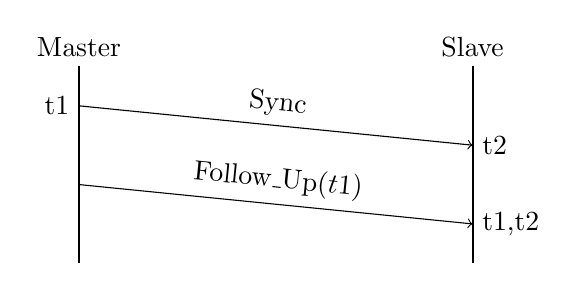
\begin{tikzpicture}
        % basic timelines master and slave
        \draw[thick] (-2.5, 0) node[anchor=south] {Master} -- (-2.5,  -2.5);
        \draw[thick] ( 2.5, 0) node[anchor=south] {Slave}  -- ( 2.5,  -2.5);
        % sync message
        \draw[->]    (-2.5, -0.5) node[left] {t1} -- ( 2.5, -1) node [midway, above, sloped]
        {Sync} node [right] {t2};
        % follow up
        \draw[->]    (-2.5, -1.5) -- ( 2.5, -2) node [midway, above, sloped]
        {Follow\_Up$\left(t1\right)$} node[right] {t1,t2};;
    \end{tikzpicture}
\end{center}
\begin{itemize}
    \item Precondition: the time the sync message takes from master to slave is known
    \item The clocks are at the same absolute time if $t2 - peerdelay = t1$ (with some tolerance)
    \item This is repeated over and over. So you can also adjust the $speed$ of the clock
\end{itemize}
\end{frame}

\begin{frame}
\frametitle{Peer delay calculation}
\begin{center}
    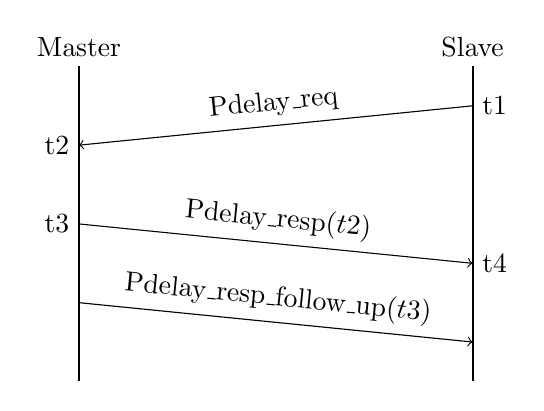
\begin{tikzpicture}
        % basic timelines master and slave
        \draw[thick] (-2.5, 0) node[anchor=south] {Master} -- (-2.5,  -4);
        \draw[thick] ( 2.5, 0) node[anchor=south] {Slave}  -- ( 2.5,  -4);
        % pdelay req
        \draw[->]    (2.5, -0.5) node[right] {t1} -- (-2.5, -1) node [midway, above, sloped]
        {Pdelay\_req} node [left] {t2};
        % pdelay resp
        \draw[->]    (-2.5, -2) node[left] {t3} -- ( 2.5, -2.5) node [midway, above, sloped]
        {Pdelay\_resp$\left(t2\right)$} node[right] {t4};
        % resp follow up
        \draw[->]    (-2.5, -3) -- ( 2.5, -3.5) node [midway, above, sloped]
        {Pdelay\_resp\_follow\_up$\left(t3\right)$};
    \end{tikzpicture}
\end{center}
\begin{itemize}
    \item t1: send timestamp of request
    \item t2: receive timestamp of request
    \item t3: send timestamp of response
    \item t4: receive timestamp of response
\end{itemize}
Calculation of delay: $(t4-t1) - (t3-t2)$
\end{frame}

\end{document}
